Una estaci\'on de radio muy popular recibe muchas llamadas en el d\'ia de tal forma que la probabilidad
de que una persona llame a la radio y la l\'inea de tel\'efono no este ocupada es 0.05. suponga que las
llamadas son independientes.
% Geometrica
% P = 0.05 , en promedio, 1 contesta cada 20 llamadas

\begin{itemize}
	\item Lea las siguientes preguntas y escriba sus hip\'otesis.
	\item ?`Cu\'al es la probabilidad de que la primera llamada que entre sea la d\'ecima que realiza la persona?\\
		Como en la Geometrica se realizan X + 1 experimentos para obtener ese 1 exito, para que entre la decima, nuestro $X=9$\\
		$p(X=9)\ =\ 0.03151247$\\% dgeom(9,0.05)
	\item ?`Cu\'al es la probabilidad de que sea necesario llamar mas de 15 veces para que encuentro la l\'inea desocupada?\\
		En este caso $X>15$, entonces necesitamos saber $X<=15$\\
		$P(X>15)\ =\ 1\ -\ P(X<=15)\ =\ 1\ -\ 0.5598733\ =\ 0.4401267\ $\\ %pgeom(15,0.05)
	\item ?`Cu\'al es el n\'umero esperado de llamadas que tiene que realizar una persona para hallar desocupada la l\'inea?.
		 Calcule utilizando el o los par\'ametros de la distribuci\'on y usando $\sum_{i=1}^{100}x\cdot p(x)$, comp\'arelos y explique por qu\'e la diferencia.\\
	$$\bar{x}\ =\ E(x)\ =\ \frac{1}{\lambda} =\ \frac{1}{0.05} =\ 20$$
	y si ahora comparamos  eso con:\\
	$$\sum_{i=1}^{100}x\cdot p(x)\ =\ 19.20401$$
	
	Nos podemos dar cuenta que la diferencia es de $0.8$ , el cual representa el error al calcular la esperanza tomando en cuenta solo 100 llamadas. La diferencia reside en que la formula de la esperanza considera la suma integral de todos los valores de 0 a infinito. De hecho, si en vez de calcularla con x=1 a 100, lo hacemos hasta 10000, la diferencia se reduce a $0.005$, una diferencia \'infima comparada con el valor entregado por la formula.

	\item Realice gr\'aficos de la funci\'on de densidad de probabilidad y de la funci\'on de distribuci\'on.\\
		% x<-seq(1,40)
	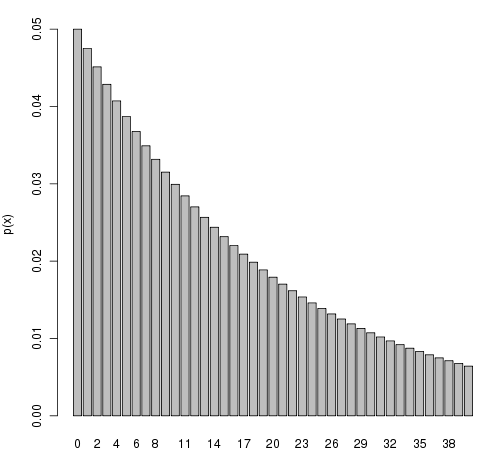
\includegraphics[scale=0.5]{images/1_2-dgeom}\\	% barplot(dgeom(x,0.05),names.arg=x)
	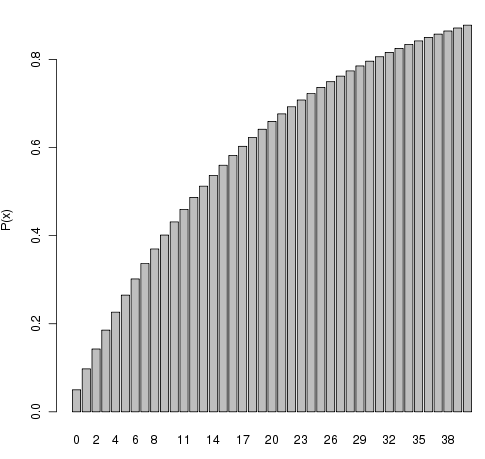
\includegraphics[scale=0.5]{images/1_2-pgeom}\\	% barplot(pgeom(x,0.05),names.arg=x)
	\item Var\'ie el o los valores de los par\'ametros de la distribuci\'on y comente lo observado en los gr\'aficos de la funci\'on de densidad y de distribuci\'on. (2 casos)\\\\

	Caso 1: Variando el $\lambda$ a $0.1$:\\
	Funci\'on de densidad de probabilidad con $\lambda\ =\ 0.1$\\
  	  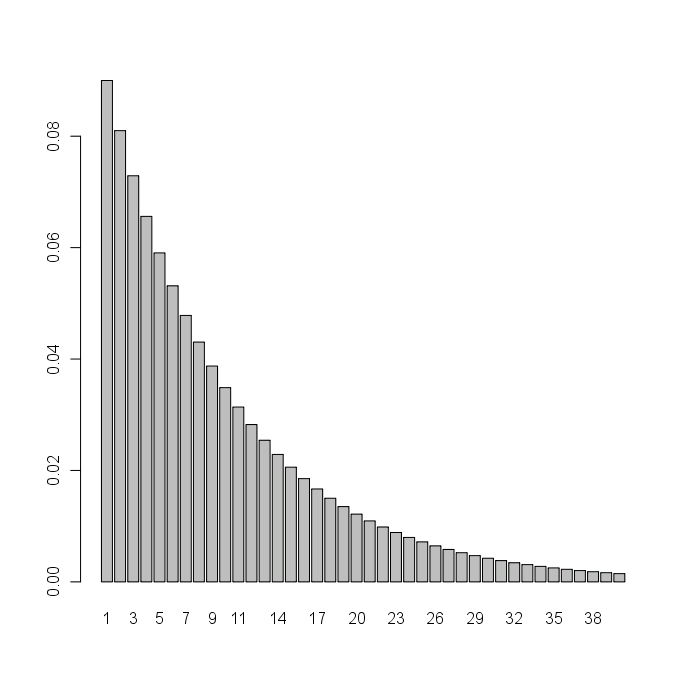
\includegraphics[width=3.3in,height=3.3in]{images/1_2-dgeom01.png}\\
	Funci\'on de distribucion con $\lambda\ =\ 0.1$\\
  	  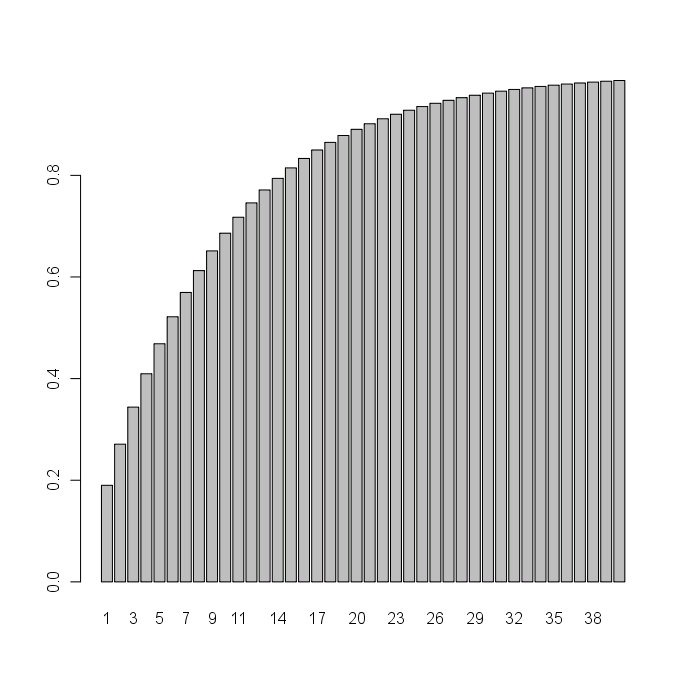
\includegraphics[width=3.3in,height=3.3in]{images/1_2-pgeom01.png}\\
	Caso 2: Variando el $\lambda$ a $0.5$:\\
	Funci\'on de densidad de probabilidad con $\lambda\ =\ 0.1$\\
  	  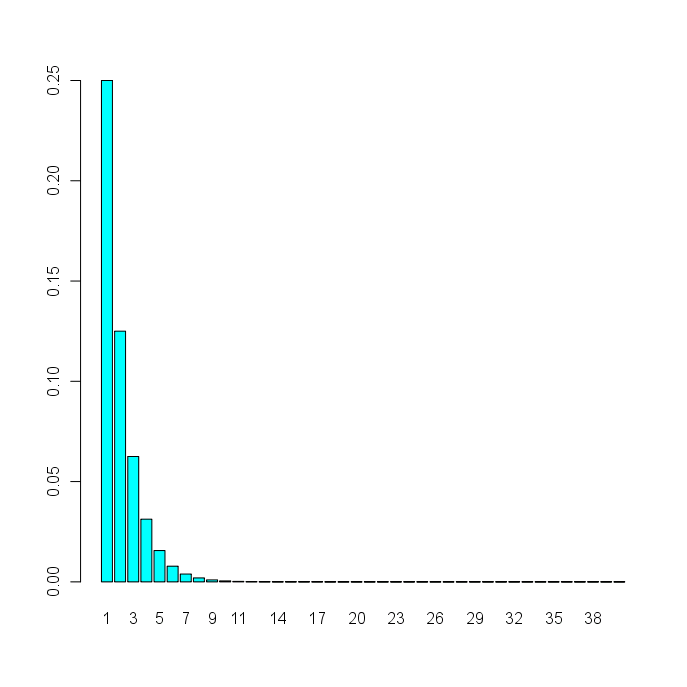
\includegraphics[width=3.3in,height=3.3in]{images/1_2-dgeom5.png}\\
	Funci\'on de distribucion con $\lambda\ =\ 0.1$\\
  	  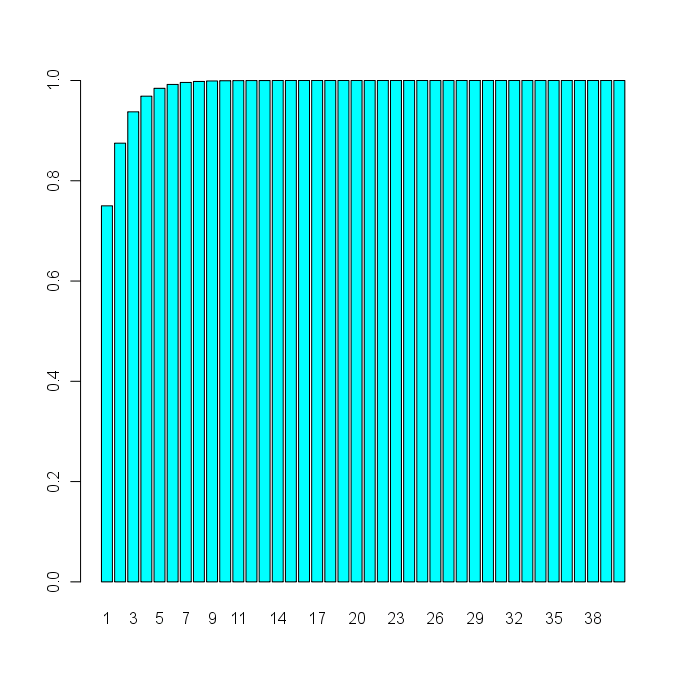
\includegraphics[width=3.3in,height=3.3in]{images/1_2-pgeom5.png}\\

	Claramente podemos observar como al aumentar el parametro $\lambda$, la funcion de densidad y distribucion tiende a comprimirse y aumentar de valor.
  De la misma forma, uno puede notar como la pendiente de las funciones se pronuncia (negativamente en la de densidad y positivamente en la de distribuci\'on) considerablemente al aumentar $\lambda$.

	


\end{itemize}
